\documentclass{beamer}
\usepackage[utf8]{inputenc}
\usepackage[croatian]{babel}
\usepackage{graphicx}
\usepackage{hyperref}
\usetheme{Madrid}

\title{Markdown}
\author{Goran Diklić, Leo Domitrović, Filip Nikolaus}
\date{7.1.2018}

\begin{document}

\maketitle

\newpage

\begin{frame}
\frametitle{Markdown}

\begin{itemize}
\item opisni markup jezik za označavanje teksta
\item jednostavan i čitak
\item Povijest:
\begin{enumerate}
\item 2004. - A. Swartz i J. Gruber kreirali sintaksu jezika Markdown
\item 2012. - standardizacija Markdown jezika - CommonMark
\item 2014. - prva inačica CommonMark-a
\item 2017. - GitHub izdaje specifikaciju za GitHub Flavored Markdown
(GFM) - baza CommonMark
\end{enumerate}

	
\end{itemize}
\end{frame}

\newpage

\begin{frame}
\frametitle{Oblikovanje teksta}
\begin{itemize}
\item podebljavanje i ukošavanje teksta
\item \emph{znakovi: * i  \_}
\item korištenje jednog znaka(* ili \_) - ukošavanje
\item korištenje dva znaka (** ili \_\_) - podebljavanje
\item kombiniranje znakova za oblikovanje riječi i rečenica
\item moguće oblikovati samo jednu riječ, nekoliko riječi ili kompletnu rečenicu
\end{itemize}
\end{frame}

\newpage

\begin{frame}
\frametitle{Podebljavanje teksta - primjeri}

\begin{figure}
{Markdown kod:}
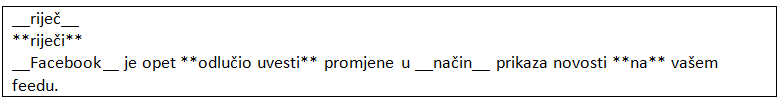
\includegraphics[width = 1.0\linewidth]{/Users/Goran/Documents/GitHub/Markdown/Podebljavanje.png}
\end{figure}

\begin{figure}
{Prikaz:}

\includegraphics[width = 1.0\linewidth]{/Users/Goran/Documents/GitHub/Markdown/Prikaz1.png}
\end{figure}

\end{frame}

\newpage

\begin{frame}
\frametitle{Ukošavanje teksta - primjeri}

\begin{figure}
{Markdown kod:}

\includegraphics[width = 1.0\linewidth]{/Users/Goran/Documents/GitHub/Markdown/Ukosavanje.png}
\end{figure}

\begin{figure}
{Prikaz:}

\includegraphics[width = 1.0\linewidth]{/Users/Goran/Documents/GitHub/Markdown/Prikaz2.png}
\end{figure}

\end{frame}


\newpage

\begin{frame}
\frametitle{Podebljavanje i ukošavanje teksta - primjeri}

\begin{figure}
{Markdown kod:} 

\includegraphics[width = 1.0\linewidth]{/Users/Goran/Documents/GitHub/Markdown/Kombinacija.png}
\end{figure}

\begin{figure}
{Prikaz:}

\includegraphics[width = 1.0\linewidth]{/Users/Goran/Documents/GitHub/Markdown/Prikaz3.png}
\end{figure}

\end{frame}

\newpage

\begin{frame}
\frametitle{Zaglavlja}
\begin{itemize}
\item strukturiranje teksta
\item služe kao naslovi i podnaslovi
\item 6 definiranih razina zaglavlja
\item definira se korištenjem znaka \# ispred naslova
\item npr. \#\# označava zaglavlje razine 2
\item drugi način zapisa zaglavlja - ukoliko cijeli naslov podcrtamo znakovima = dobijemo zaglavlje prve razine, a ukoliko naslov podcrtamo znakovima - dobijemo zaglavlje druge razine 
\item oblikovanje - podebljavanje i ukošavanje
\end{itemize}
\end{frame}

\newpage

\begin{frame}
\frametitle{Zaglavlja}
\begin{figure}
{Markdown kod:} 

\includegraphics[width = 1.0\linewidth]{/Users/Goran/Documents/GitHub/Markdown/Zaglavlja.png}
\end{figure}

\begin{figure}
{Prikaz:}

\includegraphics[width = 1.0\linewidth, height = 120pt]{/Users/Goran/Documents/GitHub/Markdown/Prikaz_zaglavlja.png}
\end{figure}
\end{frame}

\newpage

\begin{frame}
\frametitle{Zaglavlja}
\begin{figure}
{Markdown kod:} 
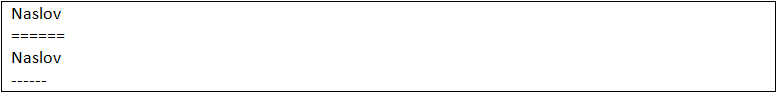
\includegraphics[width = 1.0\linewidth]{/Users/Goran/Documents/GitHub/Markdown/Zaglavlja2.png}
\end{figure}

\begin{figure}
{Prikaz:}

\includegraphics[width = 1.0\linewidth]{/Users/Goran/Documents/GitHub/Markdown/Prikaz_zaglavlja2.png}
\end{figure}
\end{frame}

\newpage

\begin{frame}
\frametitle{Oblikovanje zaglavlja}
\begin{figure}
{Markdown kod:} 

\includegraphics[width = 1.0\linewidth]{/Users/Goran/Documents/GitHub/Markdown/Oblikovanje_zaglavlja.png}
\end{figure}

\begin{figure}
{Prikaz:}

\includegraphics[width = 1.0\linewidth]{/Users/Goran/Documents/GitHub/Markdown/Prikaz_oblikovanja_zaglavlja.png}
\end{figure}
\end{frame}

\newpage

\begin{frame}
\frametitle{Poveznice}
\begin{itemize}
\item dva zapisa
\item inline - tekst koji se prikazuje korisniku unutar uglatih zagrada, a poveznica unutar oblih zagrada
\item oblik reference - poveznica je na dio dokumenta 

\end{itemize}
\end{frame}

\newpage

\begin{frame}
\frametitle{Poveznice}
\begin{figure}
{Markdown kod:} 

\includegraphics[width = 1.0\linewidth]{/Users/Goran/Documents/GitHub/Markdown/Poveznica1.png}
\end{figure}

\begin{center}
Prikaz:
\end{center}



\href{http://www.riteh.uniri.hr/}{RiTeh} \\
\href{https://www.youtube.com/?gl=HR}{YouTube}
\end{frame}

\newpage

\begin{frame}
\frametitle{Poveznice}
\begin{figure}
{Markdown kod:} 

\includegraphics[width = 1.0\linewidth]{/Users/Goran/Documents/GitHub/Markdown/Poveznica2.png}
\end{figure}

\begin{center}
Prikaz
\end{center}



\href{http://www.riteh.uniri.hr/}{RiTeh} \\
\href{https://www.youtube.com/?gl=HR}{YouTube}

\end{frame}

\newpage

\begin{frame}
\frametitle{Slike}
\begin{itemize}
\item dodavanje identično kao kod poveznica
\item jedina razlika u uskličniku koji se nalazi ispred poveznice ili reference
\item moguće postaviti poveznicu na sliku
\end{itemize}
\end{frame}

\newpage

\begin{frame}
\frametitle{Slike}
\begin{figure}
{Markdown kod:} 
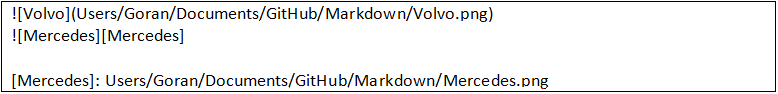
\includegraphics[width = 1.0\linewidth]{/Users/Goran/Documents/GitHub/Markdown/Slike.png}
\end{figure}

\begin{figure}
\begin{center}
{Prikaz:}
\end{center}
\begin{flushleft}
\begin{center}

\includegraphics[width = 50pt]{/Users/Goran/Documents/GitHub/Markdown/Volvo.png}
\end{center}
\end{flushleft}
\end{figure}

\begin{figure} 
\begin{flushleft}

\begin{center}

\includegraphics[width = 50pt]{/Users/Goran/Documents/GitHub/Markdown/Mercedes.png}
\end{center}
\end{flushleft}
\end{figure}

\end{frame}

\newpage

\begin{frame}
\frametitle{Poveznica na sliku}
\begin{figure}
{Markdown kod:}

\includegraphics[width = 1.0\linewidth]{/Users/Goran/Documents/GitHub/Markdown/Poveznica_na_sliku.png}
\end{figure}

\begin{figure}
\href{https://www.volvocars.com/hr}{
\includegraphics[width = 100pt]{/Users/Goran/Documents/GitHub/Markdown/Volvo.png}}
\end{figure}
\end{frame}

\newpage

\begin{frame}
\frametitle{Citati}
\begin{itemize}
\item koristi se znak $>$ ispred teksta
\end{itemize}
\begin{figure}
{Markdown kod:}

\includegraphics[width = 1.0\linewidth]{/Users/Goran/Documents/GitHub/Markdown/Citati.png}
\end{figure}

\begin{figure}
{Prikaz:}

\includegraphics[width = 1.0\linewidth]{/Users/Goran/Documents/GitHub/Markdown/Citati_prikaz.png}
\end{figure}
\end{frame}

\newpage
\begin{frame}
\frametitle{Liste}
\begin{itemize}
\item neodređene i numerirane liste
\item za neodređenu listu potrebno je staviti znak $*$ ispred svih elemenata
\item ukoliko želimo imati listu s nekoliko razina potrebno je sljedeću razinu pomaknuti za jedan razmak ili tab
\end{itemize}
\end{frame}

\newpage
\begin{frame}
\frametitle{Liste}
\begin{figure}
{Markdown kod:}

\includegraphics[width = 1.0\linewidth]{/Users/Goran/Documents/GitHub/Markdown/Neuredene_liste.png}
\end{figure}

\begin{figure}
{Prikaz:}

\includegraphics[width = 1.0\linewidth]{/Users/Goran/Documents/GitHub/Markdown/Neuredene_liste_prikaz.png}
\end{figure}
\end{frame}

\newpage
\begin{frame}
\frametitle{Liste}
\begin{figure}
{Markdown kod:}

\includegraphics[width = 1.0\linewidth]{/Users/Goran/Documents/GitHub/Markdown/Numerirane_liste.png}
\end{figure}

\begin{figure}
{Prikaz:}

\includegraphics[width = 1.0\linewidth]{/Users/Goran/Documents/GitHub/Markdown/Numerirane_liste_prikaz.png}
\end{figure}
\end{frame}

\newpage
\begin{frame}
\frametitle{Blokovi koda}
\begin{itemize}
\item ukoliko se tekst pomakne za jedan razmak desno on se čita kao kod
\end{itemize}

\begin{figure}
{Markdown kod:}
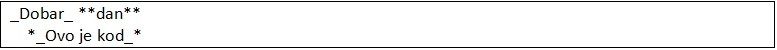
\includegraphics[width = 1.0\linewidth]{/Users/Goran/Documents/GitHub/Markdown/Blokovi_koda.png}
\end{figure}

\begin{figure}
{Prikaz:}
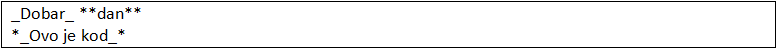
\includegraphics[width = 1.0\linewidth]{/Users/Goran/Documents/GitHub/Markdown/Blokovi_koda_prikaz.png}
\end{figure}


\end{frame}





































\end{document}